
%(BEGIN_QUESTION)
% Copyright 2006, Tony R. Kuphaldt, released under the Creative Commons Attribution License (v 1.0)
% This means you may do almost anything with this work of mine, so long as you give me proper credit

Beregn strømmen gjennom zenerdioden for de gitte verdiene av inngangsspenning (kildespenning) i denne kretsen:

$$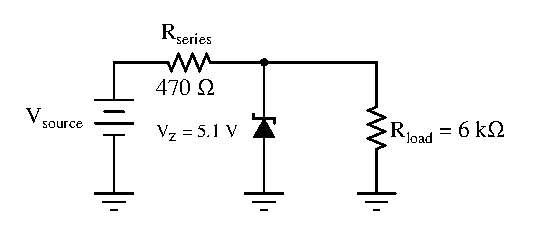
\includegraphics[width=15.5cm]{i00757x01.eps}$$

\begin{itemize}
\item{} $V_{source}$ = 25 V ; $I_{zener}$ =
\item{} $V_{source}$ = 20 V ; $I_{zener}$ =
\item{} $V_{source}$ = 15 V ; $I_{zener}$ =
\item{} $V_{source}$ = 10 V ; $I_{zener}$ =
\item{} $V_{source}$ = 5 V ; $I_{zener}$ =
\end{itemize}

Ser du noen sammenheng mellom kildespenning og zenerstrøm? Hvis ja, forklar hva denne sammenhengen er.

\underbar{file i00757}
%(END_QUESTION)





%(BEGIN_ANSWER)

Når kildespenningen synker, synker også strømmen gjennom zenerdioden:

\begin{itemize}
\item{} $V_{source}$ = 25 V ; $I_{zener}$ = 41.49 mA
\item{} $V_{source}$ = 20 V ; $I_{zener}$ = 30.85 mA
\item{} $V_{source}$ = 15 V ; $I_{zener}$ = 20.21 mA
\item{} $V_{source}$ = 10 V ; $I_{zener}$ = 9.58 mA
\item{} $V_{source}$ = 5 V ; $I_{zener}$ = 0 mA
\end{itemize}

Merk at de beregnede svarene her ikke vil samsvare {\it helt} nøyaktig med en virkelig zenerdiodemodell, fordi zenerdioder ofte taper strøm gradvis når påtrykt spenning nærmer seg zenerspenningen, i stedet for at strømmen faller brått til null slik en enklere modell predikerer.

%(END_ANSWER)





%(BEGIN_NOTES)

Denne øvelsen i strømberegning skal få studenter til å se den inverse sammenhengen mellom inngangsspenning og zenerstrøm: zenerdioden regulerer spenning ved å opptre som en parasittlast med varierende størrelse. Enkelt sagt belaster dioden kretsen så mye som nødvendig for å holde spenningen stabil over lastterminalene.

%INDEX% Elektronikkrepetisjon: spenningsregulator med zenerdiode

%(END_NOTES)


